\documentclass{article}
\usepackage[paperwidth=3in,paperheight=4.6in,margin=0in]{geometry}
\usepackage{mathptmx}%{times}
\usepackage{graphicx}
\usepackage{siunitx}
\usepackage[absolute,overlay]{textpos}

\setlength{\parindent}{0pt}
\begin{document}
\begin{textblock}{1}(2.5,0.4)
\normalsize
(a)
\end{textblock}
\footnotesize
\hspace{0.15in}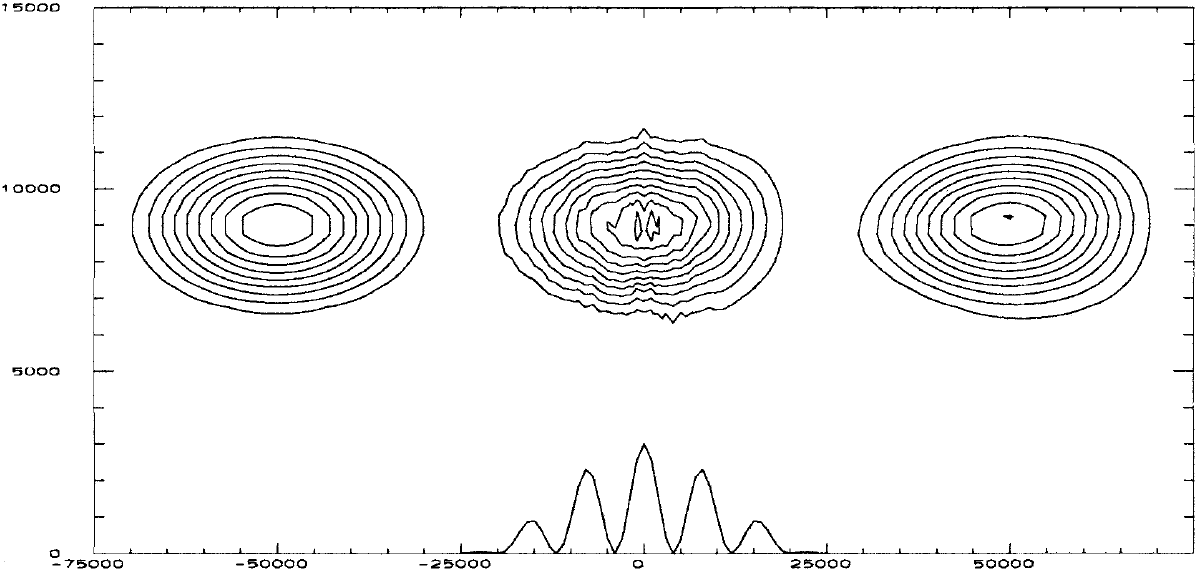
\includegraphics[width=2.75in]{img/schaer-btf-4thorder.png}

\begin{textblock}{1}(2.5,5.5)
\normalsize
(b)
\end{textblock}
\input{../advectTracer-horizontal-btf-cubicUpwindCPCFit-divFree/tracer-contour-y-only}

\begin{textblock}{1}(2.5,10.3)
\normalsize
(c)
\end{textblock}
\input{../advectTracer-horizontal-snapCol-cubicUpwindCPCFit-divFree/tracer-contour}
\end{document}
